\documentclass{mcmthesis}
\mcmsetup{CTeX = false,   % 使用 CTeX 套装时,设置为 true
        tcn = 2308935, problem = B,
        sheet = false, titleinsheet = false, keywordsinsheet = false,
        titlepage = false, abstract = true}
\usepackage{newtxtext}%\usepackage{palatino}
\usepackage{lipsum}
\title{Bringing wildlife back to Masai Mara}
\author{Your Name}
\date{\today}
\usepackage{indentfirst}
\usepackage{multirow}
\usepackage{multicol}
\usepackage{arydshln}
\usepackage{leftidx}
\usepackage{float}
\usepackage{graphicx}
\usepackage{setspace}
\usepackage[shortlabels]{enumitem}
\usepackage{booktabs}
\usepackage{array} 
\newtheorem{thm}{Theorem}[section]
\usepackage{cite}
\usepackage{hyperref}
\usepackage{booktabs}
\numberwithin{figure}{section}
\numberwithin{table}{section}
\numberwithin{equation}{section}
\usepackage{subfigure}
\fancyhead[R]{Student Name: Zhan Ruixin}
%\usepackage{parskip}
\renewcommand{\headrulewidth}{0pt}
\begin{document}
\begin{abstract}
	Forests are disappearing, natural resources are dwindling, and wildlife is being displaced. We are saddened that human activity is expanding to every corner of the planet, and human civilization is flourishing. Wildlife is also declining, a case in point being the Masai Mara region. A model for balancing the interests of humans and wildlife in the  \textbf{Masai Mara region} must be developed to achieve harmony between humans and nature and return wildlife to their rightful homes. 

	In order to achieve this, several models have been developed. 
	
	Model I: Model I is a \textbf{Grid-Method model}. As can be seen from previous articles, Grid-Method is an important method for studying territorial issues. Based on information about the distribution of animals in the Masai Mara National Reserve, we found that the distribution of wildlife is mainly influenced by \textbf{water sources} and \textbf{human activities} (livestock farming in the area). Therefore, defined the \textbf{environmental sensitivity K} based on these two factors and divided the area according to the actual geographical situation, calculating the K values for each area, the results of which are shown in Table \ref{F 5.1}. Finally, the reserve was successfully divided into seven area, and three different Zone were defined. The results are shown in Figure \ref{F 5.3}.
	
	Model II: Model II is a \textbf{composite model} that combines the \textbf{Logistic model} with a \textbf{Differential equation model} of human-nature balance. The model is based on Model 1 and is calculated for the specific case of the Masai Mara National Reserve. The Logistic model can be seen in Equation \ref{E 5.2} which is possible to \textbf{predict the change} in the animal population over time, as shown in Figure \ref{F 5.4}. And to measure the economic situation of the area, we have created a Differential equation model concerning tourism, and human activity was developed to describe the \textbf{relationship} between the current regional economy and the number of species.
	
	The human-nature equilibrium model combines both of these models, as shown in Equation \ref{E 5.6}. It is possible to predict when the wildlife population will reach its maximum under human influence and to predict the economic scenario, as shown in Figure \ref{F 5.5}. Based on the projected results generated by the model, a range of potential policies are proposed for different regions to verify their feasibility.
	
	Model III: Model III is an \textbf{Entropy-weighted evaluation model} used to select and rank the appropriate policies for each region. The secular length of Model II predictions is defined as ten years, and the predicted results are obtained. Through the calculation of this model, we determined that the most suitable policy for Masai Mara National Reserve is: \textbf{Restricting livestock farming and expanding protected area.}
	
	In addition, we applied the Model II to Serengeti National Park in Tanzania, where the maximum number of organisms was reached after 28 years, as shown in Figure \ref{F 7.2}, which is consistent with the actual situation and proves that the model is \textbf{highly generalizable} and can be used in other areas.
	
	Finally, a \textbf{sensitivity analysis} was carried out on model II (the equilibrium model) to investigate the extent to which varying the parameters (a, r, $\alpha$, $\beta$) affected the results. Three of the parameters (a, r, $\alpha$) were found to have a significant effect, and the results are shown in Section 8.
	
	
	
	
	\begin{keywords} Grid-Method model, Environmental sensitivity, Differential equation model Logistic model, Entropy-weighted evaluation model


\end{keywords}
\end{abstract}
\maketitle
%\thispagestyle{empty}
%\newpage
%\tableofcontents
%\thispagestyle{empty}
%\newpage
%%% Generate the Memorandum, if it's needed.
%% \memoto{\LaTeX{}studio}
%% \memofrom{Liam Huang}
%% \memosubject{Happy \TeX{}ing!}
%% \memodate{\today}
%% \logo{\LARGE I'm pretending to be a LOGO!}
%% \begin{memo}[Memorandum]
%%   \lipsum[1-3]
%% \end{memo}x
%%
\setcounter{page}{1}


%% 以下为正文


\section{Introduction}

\subsection{Problem Background}

"According to the International Union for Conservation of Nature (IUCN), more than 28,000 species are currently considered to be endangered". Increasing population growth and human activities of urbanisation, industrialisation and agriculture are gradually eating into and crowding out wildlife's habitat. The decline in numbers can be seen in Figure \ref{F 1.1} below. In order to counteract the decreasing species diversity, nature reserves have been established. In recent years, however, some ecological reserves have been affected, including the Masai Mara National Reserve in Kenya.

\begin{figure}[htp]
	\centering
	\begin{minipage}[t]{0.48\linewidth}
	\centering
	\includegraphics[width=0.7\linewidth]{"figures/F 1.1"}
	\caption{Decline of wildlife species in the word [https://ourworldindata.org/biodiversity]}
	\label{F 1.1}
\end{minipage}\hfill
	\begin{minipage}[t]{0.48\linewidth}
\centering
\includegraphics[width=0.7\linewidth]{"figures/F 1.2"}
\caption{Decline of wildlife biomass
		[https://journals.plos.org/plosone/article?id=10.1371]}
\label{F 1.2}
\end{minipage}\hfill
\end{figure}

Figure \ref{F 1.2} shows the change in wildlife in Kenya from 1977 to 2013, and it is distressing to note the rapid decline in wildlife biomass in this area, and the trend in Masai Mara National Reserve, an important area for wildlife in Kenya, is clearly in line with this. In response to this fact, it is imperative and urgent that a policy is put in place to reduce the impact of human activities around the nature reserve and to pursue a balance between humans and nature.

\subsection{Restatement of the problem}

An analysis of the background to the problem and a review of the actual situation in Masai Mara National Reserve with regard to the balance between man and nature, the restate of the problem can be expressed as follows:
\begin{itemize}
	\item[\ding{212}] The protected areas are divided according to the characteristics of the different areas in the reserve and modelled for their regional characteristics to predict the optimal combination of human and wildlife populations, balancing human development and nature conservation. And based on this result different specific policies are developed for different areas.
    \item[\ding{212}] Build a mathematical model to determine the plans for the various areas of the Massai Mara, taking into consideration the effects on the economy and human-animal interaction.
	\item[\ding{212}] Base on the model,develop a methodology to rank outcomes of various plans and determine the best plan.
	\item[\ding{212}] Considering the certainty and the effect of long-term trends and the usability of proposed plan.
    \item[\ding{212}] Considering the results obtained above, prepare two pages non-technical report and submit to Kenyan Tourism and Wildlife Committee.
\end{itemize}

\subsection{Literature Review}

The main issue in this situation is how to achieve a balance between people and nature around nature reserves. In recent years, with the growing interest in nature reserves, there has been a growing number of surveys on nature reserves, including the Masai Mara National Reserve.

\begin{figure}[htbp]
	\centering
	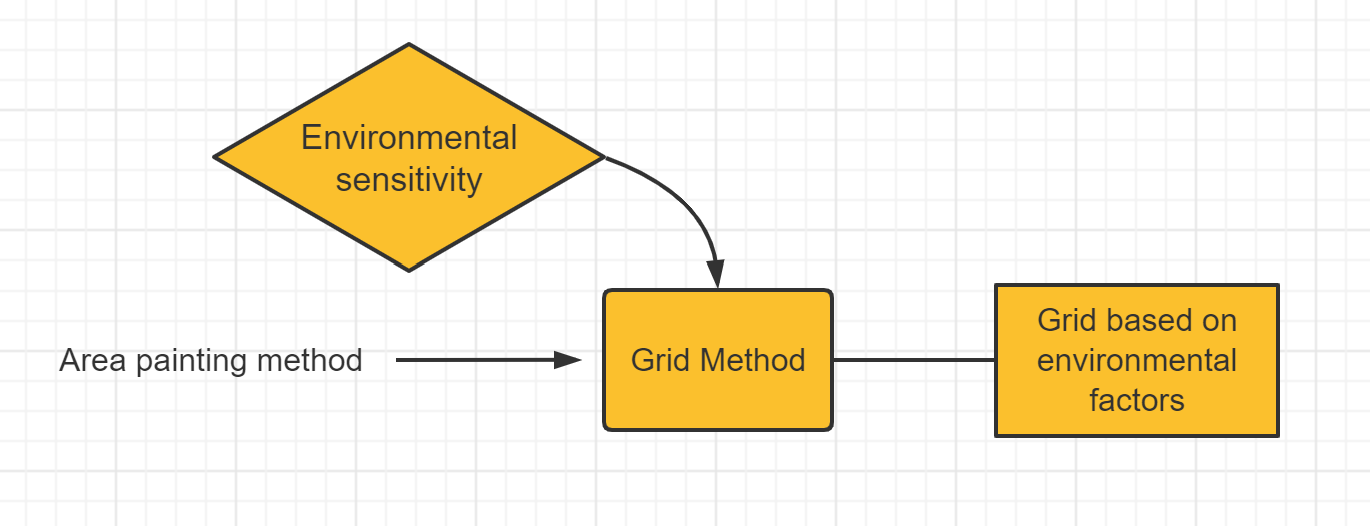
\includegraphics[width=0.5\linewidth]{./figures/review.png}
	\caption{Long-term trend}
	\label{F 1.3}
\end{figure}



\begin{itemize}
	\item The delineation of areas by grid is an important method for studying the problem of area delineation, by which areas with different characteristics are distinguished; at the same time, because planning for a three-dimensional space would make the model too complex, more authors choose to use a two-dimensional model \cite{1}. And for environmental issues, ecological sensitivity can be used as the basis for dividing the grid, and the environment's can be evaluated comprehensively through different environmental factors.\cite{2}
	\item According to the results of Nina's survey of wildlife in the area, the distribution of wildlife in the area is mainly influenced by the location of water sources and human livestock activities.\cite{1}

\end{itemize}

\subsection{Our Work}

%This issue required us to identify and evaluate policies for different areas following zoning and to demonstrate that the policies could be applied to other nature reserves. The main points of our work include the following:

\begin{figure}[htbp]
	\centering
	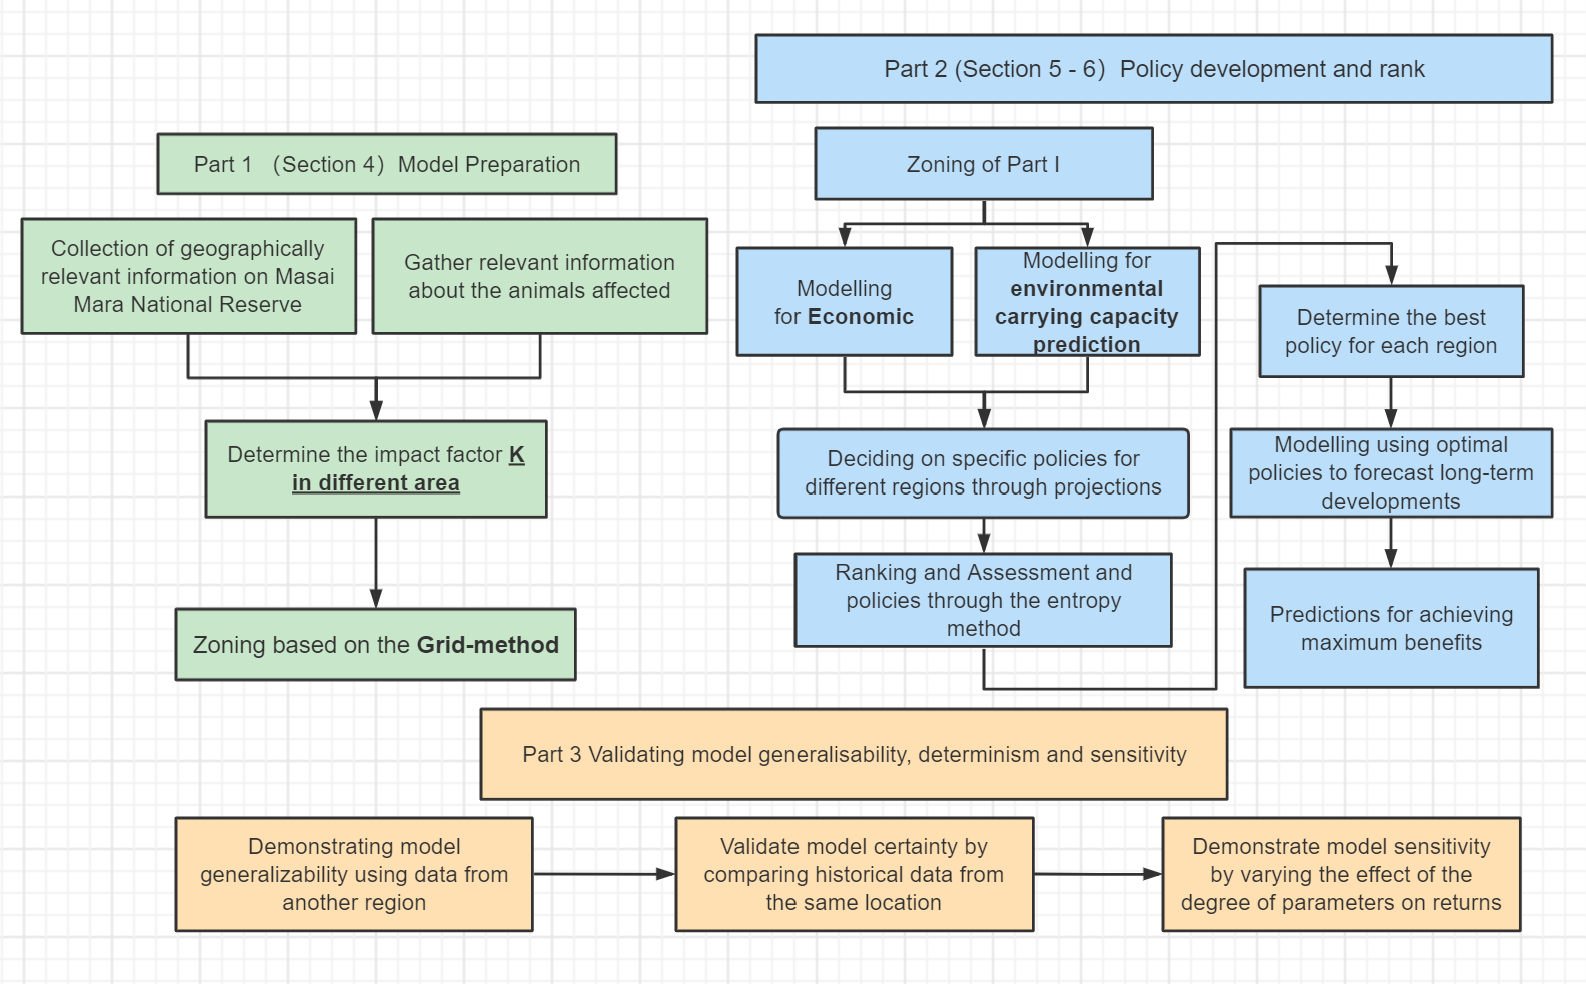
\includegraphics[width=0.85\linewidth]{./figures/our.png}
	\caption{The flow chart}
	\label{F 1.4}
\end{figure}

\section{Assumption and Explanations}

Due to the complexity of the actual problem, it is not possible to consider the full range of factors of the problem in the model. Therefore, the model developed below is based on the following assumptions:

\begin{itemize}
	\item Assumption 1: The extent of the nature reserve is the area drawn in Figure 4.1. \\
	Explanation: Because the situation at the edge of the nature reserve is more complex and the boundary itself is not clear. Using the quadrilateral in the figure as the extent of the nature reserve facilitates subsequent modelling and has little impact on the size of the area.
	\item Assumption 2: Animal populations in protected areas are influenced only by water distribution and human activity.
	\\
	Explanation: The results of the Nina survey show that these two factors are the main ones and that considering only water distribution and human activity helps to simplify the model and has a smaller impact on the results.
	\item Assumption 3: The value of latitude and longitude is used as the only measure of distance. The meaning of all coordinates below is (latitude, longitude).
	\\
	Explanation: As previously mentioned in section 1.3, it is possible to convert space into a two-dimensional plane. On this basis, a change in the value of latitude and longitude can be an accurate representation of distance.
	\item Assumption 4: All information collected during the problem solving process is accurate and available.
	\\
	Explanation: All data can be found in specific sources that prove their availability.
\end{itemize}

\section{Notations}


\begin{table}[]
	\normalsize
	\renewcommand\arraystretch{1.25}
	\centering
	\caption{Symbol description}
	\setlength{\tabcolsep}{18mm}
    \large
% Please add the following required packages to your document preamble:
% \usepackage{booktabs}
	\begin{tabular}{@{}ccc@{}}
		\toprule
		Symbol &  & Description                                         \\ \midrule
		$K_{livestock}$   &  & Human impact factor \\  
        $K_{wild}$   &  & Water impact factor                                             \\
		$K$   &  &  Area factors based on the grid method                                     \\
		$X_0$      &  & Initial number of animals                                   \\
		$X_m$     &  & Environmental carrying capacity                                       \\
		x    &  & Number of animals\\
        r    &  & Initial natural growth rate                                        \\
		a     &  &   Percentage increase in area of human activity                \\
		$\alpha$    &  & Protected area value factor                             \\
		$\beta$      &  & Value factor for livestock areas                               \\
		t     &  & Year            \\
		S     &  & Benefit of the economic model           \\
 \bottomrule
	\end{tabular}
\end{table}




\section{Model Preparation}

\subsection{Data Overview}
The problem was solved for Masai Mara National Reserve and Masai Mara National Park, but no information was given about these two areas. The analysis of the problem shows that it is inevitable to collect geographical and faunal information about the area in order to solve subsequent problems, and that visualisation can make this data more readable.

\subsubsection{Data Collection}


\subsubsection{Data Summary}

 The search resulted in the collection of maps of Masai Mara National Reserve and Masai Mara National park Figure \ref{F 4.1}, and also revealed that the human settlements adjacent to the nature reserve are pastoral areas. The conflict between pastoral areas and nature reserves is therefore the main issue to be discussed.  
\begin{figure}
	\centering
	\includegraphics[width=0.5\linewidth]{"figures/F4.1 National park map"}
	\caption{The National park map [https://www.maasaimarakenyapark.com/information/location/]}
	\label{F 4.1}
\end{figure}


 This is because the boundary line of the nature reserve is unclear and too irregular. As mentioned in Part II, in order to simplify the model, the conservation was subsequently modelled and analysed as a quadrilateral area by taking and fitting the latitude and longitude to the edge portion of the reserve. The images were fitted in Matlab by calculating the latitude and longitude of four points, A (-1.2644, 35.0457), B (-1.6068, 35.3913), C (-1.4108, 34.7604) and D (-1.7233, 35.3298), and visualised and labelled with key locations using maps, the results of which are shown in Figure F \ref{F 4.2}. The procedure for fitting the calculations can be found in Appendix 1.
 
 \begin{figure}[htp]
 	\centering
 	\begin{minipage}[t]{0.48\linewidth}
 		\centering
 		\includegraphics[width=0.7\linewidth]{"figures/F 4.2"}
 		\caption{Masai Mara National Reserve in Matlab }
 		\label{F 4.2}
 	\end{minipage}\hfill
 	\begin{minipage}[t]{0.48\linewidth}
 		\centering
 		\includegraphics[width=0.7\linewidth]{"figures/F4.3 Masai area Map"}
 		\caption{Masai Mara National Reserve in Map}
 		\label{F 4.3}
 	\end{minipage}\hfill
 \end{figure}
 
 According to the Google Map it can be seen that there are several human towns near the line AB, therefore defining the right side of the line as an area of human activity. Point E (the confluence of the three rivers) within the protected area is also defined as the water source.
 
\section{A model of balance between human and nature}

\subsection{Grid-Method based zoning}
Nature reserves are large, and the distribution of natural resources and fauna varies somewhat between different areas of the reserve. In order to develop policies for the characteristics of the different areas, it is necessary first to divide the nature reserves into zones. Previous articles mentioned that areas could be divided into rasters, and each small raster can be analyzed separately \cite{1}; ecological sensitivity coefficients can also be defined to quantify the differences between different areas (article Guangxi).
\\
To explore the balance between wildlife, natural resources and human activities: human activities and water sources are used to influence ecological sensitivity. The response to environmental influences is through the distance from wildlife to the water source (point E), and the response to influences by human activities is through the distance from wildlife to AB.

\subsubsection{Anthropogenic impact factors and Water impact factors}
The livestock area is defined as an area of human activity, and the human activity factor $K_H$ is discussed according to the distance from AB. The three equivalents of the lines AC and BD are found and connected. The protected area is divided into three parts, representing different levels of human activity, with the further away from the livestock area, the less human activity is affected. The results of the classification are shown in Figure 5.1.
\\
The water source is defined as the confluence of three rivers, E (-1.43280, 35.06375), and the water impact factor $K_W$ is discussed around point E. The area is divided into three parts according to the size of the protected area. The three parts represent the different levels of impact on the water source, with the farther away from the water, the less impact it has. This is shown in Figure 5.2.
 \begin{figure}[htp]
	\centering
	\begin{minipage}[t]{0.48\linewidth}
		\centering
		\includegraphics[width=0.7\linewidth]{"figures/F5.1Human Factor"}
		\caption{Anthropogenic impact Factor }
		\label{F 5.1}
	\end{minipage}\hfill
	\begin{minipage}[t]{0.48\linewidth}
		\centering
		\includegraphics[width=0.7\linewidth]{"figures/F5.2water factor"}
		\caption{Water impact factors}
		\label{F 5.2}
	\end{minipage}\hfill
\end{figure}

The following weighting analysis was carried out on the anthropogenic and water impact factors, with Bhola mentioning that the human impact had reduced the number of animals moving in the area by $50\%$ between 1970 and 2000\cite{1}. The $K_H$ for the three areas was therefore specified to be [1, 1.25, 1.5] from near to far. The article also refers to the biological density of the area during the wet and dry seasons, and it can be seen that the animal density in the wet season is twice as high as in the dry season. Therefore, the $K_H$ for the three areas are [2, 1.5, 1] from near to far. 


The environmental sensitivity K can be calculated by equation \ref{Eq 5.1}.
\begin{equation}
K=K_{water}*K_{human}
\label{Eq 5.1}
\end{equation}

\subsubsection{Zoning by environmental sensitivity}
According to the division rules in section 5.1.1, the whole protected area can be divided into eight zones, and 7 types of K values (1, 1.25, 1.5, 1.875, 2, 2.25, 2.5) are obtained. Based on the size of the K values, the protected area was divided into three zones, representing the magnitude of the impact by environmental sensitivity. The results are shown in Table \ref{T 5.1} and Figure \ref{F 5.3}. Follow-up questions will be based on the above zoning.

\begin{table}[htp]
	\centering
	\normalsize
	\renewcommand\arraystretch{1.5}
    \caption{The date of different types of rider}
    \label{T 5.1}
    \setlength{\tabcolsep}{12mm}
\begin{tabular}{@{}cccc@{}}
	\toprule
	\textbf{Group} & \textbf{Factor} & \textbf{Color} & \textbf{Effect} \\ \midrule
	Zone A        & 1.0-1.25        & Green          & Low             \\
	Zone B        & 1.5-2.0         & Yellow         & Medium          \\
	Zone C        & 2.0-2.5         & Red            & High            \\ \bottomrule
\end{tabular}
\end{table}

\begin{figure}
	\centering
	\includegraphics[width=0.5\linewidth]{"figures/F5.3 Zoneing"}
	\caption{Zone Map}
	\label{F 5.3}
\end{figure}

\subsection{Logistic regression based on Grid-Method}
The Logistic model is a population growth model, optimised by an exponential growth model. The growth rate of animal populations in nature cannot always be a constant number growing indefinitely and is often subject to natural conditions and human factors. These factors have a negative impact on the growth rate of animals and are taken into account in the Logistic Sturt model.
\\
The following logistic equation (\ref{E 5.2}) was developed to explore the effect of natural sensitivity (K) on the rate of animal self-enhancement (r), using Zone A as an example. In his article, Ogutu investigated the population density of 12 representative species of animals in Masai Mara National Reserve \cite{3} . The average population density was 7 animals per species per square kilometer, so it was assumed that the density of animals in the area was 84 animals per square kilometer. In order to obtain the maximum environmental carrying capacity of the area, K=1.25 in zone A was used, and the number of animals stopped growing when the area reached the environmental carrying capacity($X_m$).

\begin{equation}
	\large{
		\left\{ \begin{array}{l}
			\frac{dx}{dt}=r*x*\left( 1-\frac{x}{X_m} \right)\\
			X_m=84*K\\
		\end{array} \right.} 
	\label{E 5.2}
\end{equation}
This differential equation represents the relationship between the number of animals X and time t. The curve of the growth of the number of animals with time can be obtained when the remaining variables are determined. Moreover, regions correspond to $X_m$ versus K, as shown in Table \ref{T 5.2}.

\begin{table}[thb]
	\normalsize
	\renewcommand\arraystretch{1.07}
	\centering
	\caption{The table of different factor in different zone}
	\label{T 5.2}
	\setlength{\tabcolsep}{14mm}
	\begin{tabular}{ccc}
		\hline
		Zone & K     & $X_m$ \\ \hline
		A     & 1.25  & 105      \\
		B     & 1.875 & 158      \\
		C     & 2.5   & 210      \\ \hline
	\end{tabular}
\end{table}

To conclude, the differential equations for each of the three regions were solved, and the results are shown in Figure \ref{F 5.4}. The figure shows that the larger the natural growth rate (r) of the model, the larger maximum environmental carrying capacity ($X_m$).

\begin{figure}
	\centering
	\includegraphics[width=0.5\linewidth]{"figures/F 5.4"}
	\caption{The result of logistic equation in 3 Zone}
	\label{F 5.4}
\end{figure}

\subsection{Economic models based on Grid-Method}
To precisely quantify the economic benefits, we used Equation E \ref{E 5.3} for this calculation. Where $\alpha$ represents the wildlife viewing coefficient, which represents the benefit from wildlife at 3.5K USD per $km^2$, and $\beta$ represents the livestock benefit coefficient, using Kenya's total agricultural GDP (110.35Billion USD) divided by Kenya's total land area (569,140$km^2$) to obtain the Kenya Bureau of Statistics economic efficiency factor of 4.9K USD per $km^2$ \cite{5}.
\large{
\begin{equation}
	S=S_{reserve}+S_{livestock}=\alpha x_{wild}+\beta x_{livestock}
	\label{E 5.3}
\end{equation}
}

For the calculation of animal numbers in protected areas, we used a logistic model to describe the trend in animal numbers over time. In order to relate the natural resources of protected areas to human activity, we defined the percentage expansion of the area by human activity per year a, i.e. the area of protected areas decreases per year by a and the area of livestock areas increases per year by a. We introduced the logistic model to obtain the following logistic model under the influence of human activity, which is Equation \ref{E 5.4}
\begin{equation}
\frac{dx}{dt}=r*x*(1-\frac{x}{x_m})*(1-a*t)
\label{E 5.4}
\end{equation}
In order to be able to use this differential equation in the economic model, we need to solve it to obtain its original function Equation E \ref{E 5.5} 

\large{
\begin{equation}
X(t)=\frac{\text{X}_{\text{m}}}{\text{e}^{\frac{a\,r\,t^2}{2}}\,\text{e}^{-r\,t}\,\left( \frac{\text{X}_{\text{m}}}{X_0}-1 \right) +1}
	\label{E 5.5}
\end{equation}
}

We then replaced $x(t)$ with the wildlife population $x_{wild}$ and $a*t$ with livestock returns $x_{livestock}$ to obtain the total economic model Equation E \ref{E 5.6}, which can be used to quantify the equilibrium relationship between protected and economic areas in a given zone A and to inform related decisions.

\large{
\begin{equation}
S=\frac{\alpha \,\text{X}_{\text{m}}}{\text{e}^{\frac{a\,r\,t^2}{2}}\,\text{e}^{-r\,t}\,\left( \frac{\text{X}_{\text{m}}}{X_0}-1 \right) +1}+\beta a\,t
\label{E 5.6}
\end{equation}
}

Taking the $x_m$ of the data set A in Section 5.1 as 105, $x_0$=42. So that r=0.07 a=0.05, take into equation A, the Figure \ref{F 5.5} shows the results.


The first Figure shows the curve of economic returns over time, which shows that in this case (a=0.05 r=0.07), the 10-year return is 198, and the maximum return is reached at year 20 (215). The second Figure shows the curve of the number of animals over time, and the analysis shows that, in this case, the number of animals after ten years is 55.

In conclusion, the analysis of both graphs shows a clear correlation between the economic return and the number of animals in this case.

\begin{figure}
	\centering
	\includegraphics[width=0.5\linewidth]{"figures/F 5.5"}
	\caption{Results of the economic model}
	\label{F 5.5}
\end{figure}

\subsection{Policies proposed for different zones}
The conflict between nature reserves and livestock areas is a complex issue that requires a combination of environmental protection and socio-economic and cultural factors. To use the economic model presented above, it is assumed that all policies affect the parameters in the economic model. There are many different kinds of policies, and depending on the parameters affected, policies can be analysed in six groups. Table \ref{T 5.3} shows the relevant information for the classification
\begin{itemize}
	\item  Policy Group 1 (Normal): Regional planning  differentiating between livestock and nature reserves.
	\item Policy Group 2 (Moderate grazing): Moderate livestock development.
	\item Policy Group 3 (Overgrazing): Overgrazing and fishing.
	\item Policy Group 4 (Returning grazing): Restricting livestock farming and expanding protected area.
	\item Policy Group 5 (Poaching (animal trade)): Encourage animal trade.
	\item Policy Group 6 (poaching and overgrazing): not only encouraging animal trade, but also expanding protected area.		
\end{itemize}

\begin{table}[htbp]
	\centering
	\setlength{\tabcolsep}{9mm}
	\caption{Policy groupings}
	\label{T 5.3}
	\begin{tabular}{cccc}
		\hline
		No & Policy Groups   & a &r \\ \hline
		1 & Normal   & 0&0.07\\
		2 & Moderate grazing    &  0.05& 0.07\\
		3 & Overgrazing   &  0.1& 0.07\\
		4 & Returning grazing  & -0.1& 0.07\\
		5 & poaching (animal trade)    &  0.05& -0.07\\
		6 & poaching and overgrazing    & 0.1&-0.07\\ \hline          
	\end{tabular}
\end{table}

The next section describes the effects of the policies in each zone and ranks the best policies for each zone using the model developed in this section.

\section{EWM-based policy comparison and choice}

\subsection{Data from the quantitative analysis of the policy}
Data for each of the three zones (A:$x_m=105$ B:$x_m=158$ C:$x_m=210$) are taken into the economic model to obtain the following data.

\subsubsection{Zone A data}

\begin{table}[htbp]
    \centering
	\caption{The data of  A}
	\label{T 6.1}
    \begin{tabular}{ccccccc}
    \hline
Policy No.   & a    & r     & S(10 year) & S(Max) & tmax(Max year) & n(Number of wild animals) \\ \hline
    1                 & 0    & 0.07  & 212                & 351.6          & 50                            & 60                        \\
    2        & 0.05 & 0.07  & 198                & 215            & 20                            & 55                        \\
    3             & 0.1  & 0.07  & 184                & 184            & 10                            & 51                        \\
    4       & -0.1 & 0.07  & 240                & 350            & 30                            & 70                        \\
    5  & 0.05 & -0.07 & 105                & 0              & 0                             & 34                        \\
    6& 0.1  & -0.07 & 122                & 0              & 0                             & 34                        \\ \hline
    \end{tabular}
\end{table}


\subsubsection{Zone B data}
\begin{table}[htbp]
	\caption{The data of Zone B}
	\label{T 6.2}
	\begin{tabular}{ccccccc}
	\hline
	Policy No. & a    & r     & S(10 year) & S(Max) & tmax(Max year) & n(Number of wild animals) \\ \hline
	1          & 0    & 0.07  & 236        & 510    & 50             & 67                        \\
	2          & 0.05 & 0.07  & 214        & 238    & 20             & 60                        \\
	3          & 0.1  & 0.07  & 193        & 193    & 10             & 53                        \\
	4          & -0.1 & 0.07  & 279        & 530    & 30             & 82                        \\
	5          & 0.05 & -0.07 & 100        & 0      & 0              & 28                        \\
	6          & 0.1  & -0.07 & 118        & 0      & 0              & 32                        \\ \hline
	\end{tabular}
\end{table}

\subsubsection{Zone C data}
\begin{table}[!]
	\caption{The data of Zone C}
	\label{T 6.3}
	\begin{tabular}{ccccccc}
	\hline
	Policy No. & a    & r     & S(10 year) & S(Max) & tmax(Max year) & n(Number of wild animals) \\ \hline
	1          & 0    & 0.07  & 250        & 656    & 50             & 71                        \\
	2          & 0.05 & 0.07  & 220        & 251    & 20             & 63                        \\
	3          & 0.1  & 0.07  & 198        & 198    & 10             & 55                        \\
	4          & -0.1 & 0.07  & 310        & 715    & 37            & 90                        \\
	5          & 0.05 & -0.07 & 96         & 0      & 0              & 27                        \\
	6          & 0.1  & -0.07 & 115        & 0      & 0              & 31                        \\ \hline
	\end{tabular}
\end{table}

\subsubsection{conclusion}
Using 10 years as the implementation time, the policy was quantified and then the data was obtained as shown in the graph.
Note that at an r value of -0.07, the number of animals is decreasing each year. At this point the maximum economic benefit over the 10 year period is the benefit in year 0.

\subsection{Finding the optimal policy}
\subsubsection{The mathematical principle of the entropy weight method}
The entropy weight method is a biased and objective approach, entropy is an indicator of uncertainty, the more the (probability) distribution of an information tends to be consistent the greater the uncertainty of the information provided, the uncertainty is greatest when the information is uniformly distributed, using the entropy method we need the following formula and matrix.

Original decision matrix D
The normalisation formula is: 
\begin{equation}
	r_{ij}=\frac{d_{ij}}{\sum_{i=1}^m{d_{ij}}} 
	\label{E 6.1}
\end{equation}
\\
The entropy formula is: 
\begin{equation}
	E_{ij}=-k\sum_{i=1}^m{r_{ij}lnr_{ij}},k=1/lnm
	\label{E 6.2}
\end{equation}
\\
Distinctness formula:
\begin{equation}
	F_j=1-E_j, 0\le F_j \le 1
	\label{E 6.3}
\end{equation}
\\
Weighting formula: 
\begin{equation}
	w_j=\frac{F_j}{\sum_{j=1}^nF_j}
	\label{E 6.4}
\end{equation}

Weighted sum formula: 
\begin{equation}
	V=R*W
	\label{E 6.5}
\end{equation}

We need the original decision matrix D = [S(10),N(human)], which S(10),N(human) is the benefit in year 10 and the number of species affected by humans in year 10 in the table above, we have 6 scenarios, so here between S(10) and N(human) in this case both attributes are benefit type attributes, so the original data will be input directly into the original decision matrix D is sufficient. After obtaining the original matrix D, in order to calculate the entropy (benefit, quantity) of the two attributes, we need to change the scale of D and use the normalisation formula to derive a normalised decision matrix R. In this case both attributes are benefit attributes, so the original decision matrix D can be entered directly. 

After obtaining the normalised decision matrix R, we use the entropy formula to determine the degree of confusion of the two attributes and obtain the column vector of entropy $E_j$ by formular \ref{E 6.2}, then according to our known column vector of entropy, we apply the differentiation formula \ref{E 6.3} to obtain the differentiation of the attributes, and finally according to the weight formula \ref{E 6.4}, we obtain the column vector of weight $W_j$. 

Finally according to the weighted sum formula \ref{E 6.5}, we obtain the combined weight (degree of superiority or inferiority) of the scheme to the target.
In our model, the algorithm has been written in matlab for the series of steps in the previous paragraph, so when we need to know the degree of superiority or inferiority of the policy, we just need to fill in the original matrix D with the number of benefits and species in the tenth year of each scenario and the result will be known.


\subsubsection{Data substitution and analysis}

The quantitative data of our policy were brought into the entropy method model to obtain the combined weights of the different scenarios in the three groups, which is $V_a ,V_b,V_c$

%These three vectors indicate the degree of superiority or inferiority of the six methods of no intervention, moderate grazing, overgrazing, returning grazing to forest, encouraging animal trade, and transitional grazing and encouraging animal trade for region A.%, respectively, as 0.198665307 0.183944376 0.170766732 0.228107168 0.105005478 0.11351094. 
%The sum of these ratios is 1. It is clear from the ratios that option 4 (returning grazing to forest) has the best short-term benefits, followed by no intervention, moderate grazing, overgrazing, transitional grazing and encouraging animal trade, and encouraging animal trade.

These three vectors indicate that for Zone A,B,C the six methods of no intervention, moderate grazing, overgrazing, returning grazing to forest, encouraging animal trade, and transitioning grazing and encouraging animal trade are the best and worst.%, respectively, at 0.207574435 0.186990173 0.166820943 0.249964152 0.087317418 0.101332879 .
The sum of these ratios is 1. It is clear from the ratios that option 4 (return of grazing to forest) has the best short-term benefits, followed by no intervention, moderate grazing, overgrazing, transitional grazing and encouraging animal trade, and encouraging animal trade.

%These three vectors indicate that for Region C, the six methods of no intervention, moderate grazing, overgrazing, returning grazing to forest, encouraging animal trade, and transitioning grazing and encouraging animal trade are superior or inferior.% by 0.2105 0.186 0.1648 0.264 0.0804 0.0943 respectively.
%The sum of these ratios is 1. It is evident from the ratios that Option 4 (returning grazing to forest) has the best short-term the best benefits, followed by no intervention, moderate grazing, overgrazing, transitional grazing and encouraging animal trade, and encouraging animal trade.

%To give a more visual representation of which method is better, we numbered the options sequentially and draw 
Here are the scatter plots of the weighted sum-options within each Zone.
These figures show the weighting of different policies affecting the economy in different Zones.

\begin{figure}[htp]
	\centering
	\begin{minipage}[t]{0.33\linewidth}
	\centering
	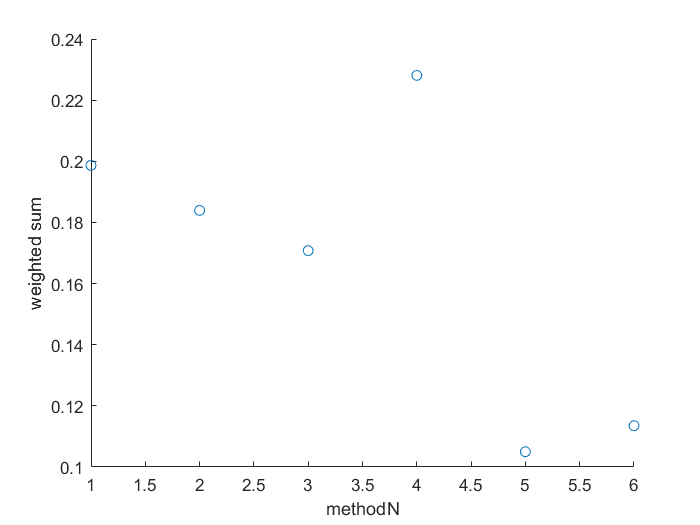
\includegraphics[width=0.7\linewidth]{./figures/Q2a.png}
	\caption{Weight of Zone A}
	\label{F 6.1}
\end{minipage}\hfill
	\begin{minipage}[t]{0.33\linewidth}
\centering
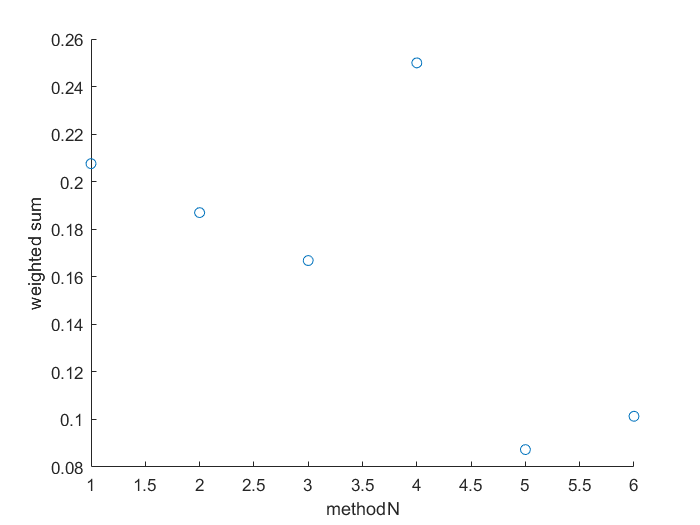
\includegraphics[width=0.7\linewidth]{./figures/Q2b.png}
\caption{Weight of Zone B
		}
\label{F 6.2}
\end{minipage}\hfill
    \begin{minipage}[t]{0.33\linewidth}
	\centering
	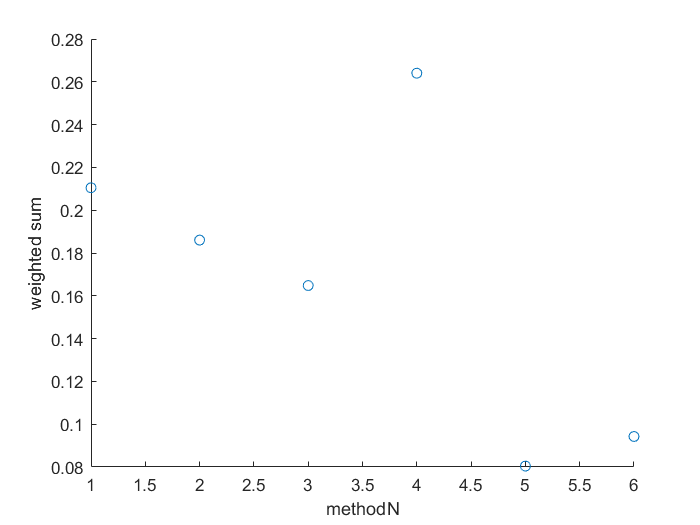
\includegraphics[width=0.7\linewidth]{./figures/Q2c.png}
	\caption{Weight of Zone C
			 }
	\label{F 6.3}
	\end{minipage}\hfill
\end{figure}




\subsection{Discussion of results}
\subsubsection{Discussion of Figure}
Figure analysis: Although the specific weighting of each option differs in each of the three zones, the level of merit (ranking) is the same in all three zones, with option 4 (returning grazing to forest) being the best, followed by no intervention, moderate grazing, overgrazing, transitional grazing and encouraging animal trade, and encouraging animal trade. So we have adopted a policy of returning grazing to forest for all three areas.
\subsubsection{Specific policies for the different zones}
Based on the analysis of the data, we should adopt a programme to reduce the negative impact of humans on animals for all three areas A,B,C. The following are the specific policies to achieve this.



For zone A, since A itself is close to the livestock boundary line, the impact of human activities on zone A can be reduced by changing the extent of the livestock boundary line, for example by reducing the area of part of the livestock zone by 1\% per year. The impact of human activities on Area A can be mitigated by including this area in the nature reserve.

To reduce the negative impact of humans, we can reduce the rate of human occupation of water resources, for example by introducing new water recycling systems to reduce pollution or waste of water resources, thus allowing animals to have more access to pure water resources.

For Area C, where there are many towns, we could reduce the industrial or domestic pollution generated by the towns in Area C by introducing new waste disposal systems, or by investing more of the money that would otherwise be spent on industrial production in the construction of animal migration camps, which would compensate for the shortfall in industrial production through the income generated by tourism, while better protecting the animals in Area C.








\section{Adaptive exploration of models}
\subsection{Long-term trends of the programme}
\subsubsection{Long-term trend images}

\begin{figure}
	\centering
	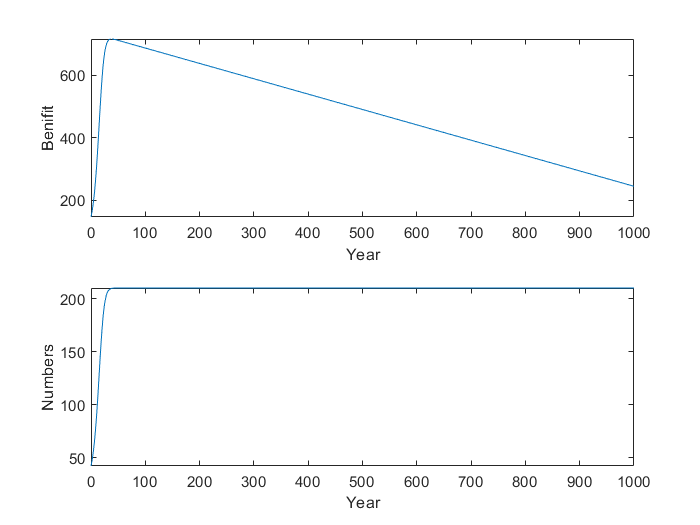
\includegraphics[width=0.5\linewidth]{./figures/Q3_1C.png}
	\caption{Long-term trend}
	\label{F 7.1}
\end{figure}



In order to observe the long-term trends of our chosen scenario, we chose the total return S and the total number of species N over the period 0-1000 years as our reference indicators, using region C as a proxy for the study.

\subsubsection{Mathematical analysis of long-term trends}
As the trends in income and species numbers are broadly similar in all three zones adopting this policy, only zone C is chosen here as a representative for analysis. Both income and animal numbers rose sharply in zone C for a short period of time after the adoption of the Reforestation Policy until the 38th year. After that the income starts to decline and the number of species remains more or less constant. The income equation shows that it is the linear term $a*\beta*t$ that leads to a linear decrease later on, while in the species population equation a only affects the growth rate, and the species population itself is close to its maximum capacity xm at year 38, so the effect of a is hardly visible after year 38.

\subsubsection{Realistic impact estimates for long-term trends}

Based on our mathematical analysis, we can tell that both income and species numbers are rising significantly in the first 38 years, which can be attributed to the fact that the adoption of the policy of returning grazing land to forestry has led to an increase in the number of visitable sites in nature reserves attracting more tourists, while at the same time, animals are subject to less human activity leading to more total accessible natural resources, thus leading to The total number of animals increased. After the 38th year, the benefits of tourism from the expansion of the reserve are less than the benefits of using the expanded area for agricultural activities, resulting in a gradual decrease in benefits. At the same time, as the total amount of natural resources available to animals in a fixed area is limited, animal populations remain more or less constant as they converge to the maximum number of species.

\subsection{Widespread use of models}

There are many wildlife conservation centres similar to those in the Masai Mara, such as Serengeti National Park in Tanzania, savo West National Park in Kenya, Kruger National Park in South Africa, kavango Delta in Botswana.
Here we apply our model to the Serengeti as an example.



\subsubsection{Parameter selection} 
When we use this model for different wildlife management areas, we only need to consider the following parameters
$\alpha$: tourism yield index in ($KUSD/km^2$)
$\beta$: agricultural return index in ($KUSD/km^2$)
$X_m$: maximum number of species
Other parameters, such as r, $x_0$, a, are universal data determined from extensive studies, (0.07,42,-0.1) and need not be considered here


\subsubsection{Parameter calculations}
When we apply to the Serengeti Nature Reserve in Tanzania
calculating $\alpha$, we need to know the total gdp of tourism in the country and the land area of the country, citing statita. \cite{6}
To calculate the $\alpha$, we need to know the country's total tourism GDP and the country's land area, citing statita \cite{7} and the land area in worldbank \cite{7}, divided by the two to find the tourism return index $\alpha$ = 1.7. To calculate the $\beta$, we need to know the country's Agricultural GDP and land area, cited from tradingeconmics \cite{8} and worldbank \cite{9} and divide the two to obtain $\beta$=3.1 ($KUSD/km^2$). When considering the number of species in the Gueren Seti, we do not take into account regional factors, so we take xm = 84 without multiplying by any scale factor.

\subsubsection{Simulation application and analysis of the model}
The parameters we obtained were taken into the model and simulations were carried out to find the maximum benefit and the maximum number of species in the Serengeti at year 28. The derivation shows that the Serengeti will have the highest number of species and the highest return at year 28, with a specific value of 83 species per $km^2$ and a return of 132.838 $KUSD/km^2$.

\begin{figure}
	\centering
	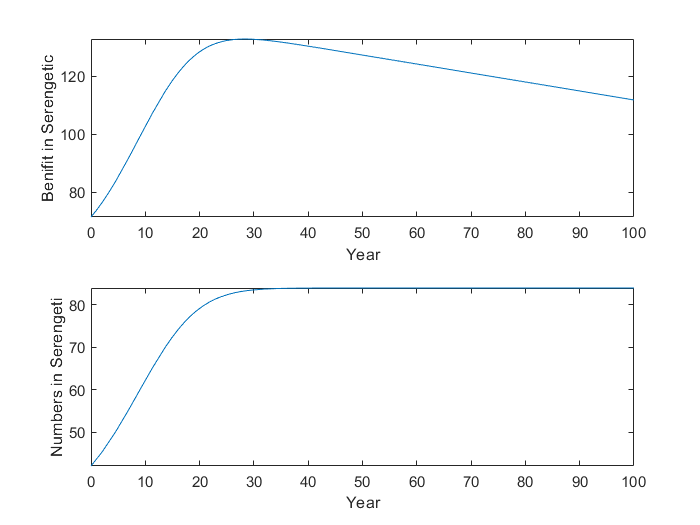
\includegraphics[width=0.5\linewidth]{./figures/Q3.png}
	\caption{Simulation result}
	\label{F 7.2}
\end{figure}


\subsubsection{Certainty of the long-term results of the model}
Because Maasai Mara populations have been declining over decades, we need to use data on the presence of population growth in other similar areas to demonstrate the certainty of our model's long-term results. 

Here we consider the Serengeti Nature Reserve, where we have more historical data. For the Serengeti, we have historical data on the number of species from 1950-2010, with particular attention to the fact that the Serengeti was plagued by viruses until the 1950s and animal numbers remained low.\cite{10}

Animal vaccination campaigns were carried out after the 1950s, with species numbers peaking in 1977, and only after 1977 did species numbers decline due to human activities. This is similar to the situation described by the parameters x0 (number of species after the dry season and before the start of the rainy season) and a = -0.1 (positive contribution of humans to species growth) in our model, so we can use historical data from the Serengeti to compare with our application of the model to the Serengeti to determine the certainty of the long-term results of our model.


\begin{figure}
	\centering
	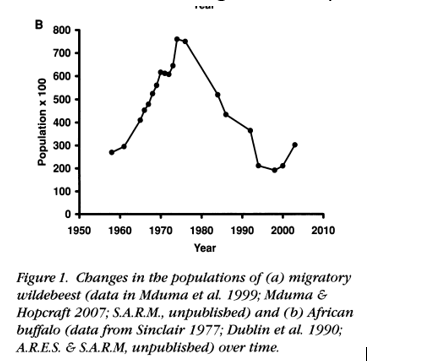
\includegraphics[width=0.5\linewidth]{./figures/Q3P.png}
	\caption{Paper result}
	\label{F 7.3}
\end{figure}


The simulation results show that the Serengeti will reach a population maximum after 28 years following the adoption of a regression policy, while historical data show that the Serengeti will take 27 years to reach a population maximum under similar circumstances. This is almost identical to the results obtained by our model, so we believe that the certainty of the model's long-term results is high.

\section{Sensitivity analysis}
\subsection{Sensitivity analysis methods and parameters}
We test the effect of different parameters on the output S (the tenth decade of interest), while we control for other variables to remain constant during the process, and subsequently draw images of the different parameters versus S to determine sensitivity.


\begin{figure}[htbp]
	\centering
	\begin{minipage}[t]{0.48\linewidth}
	\centering
	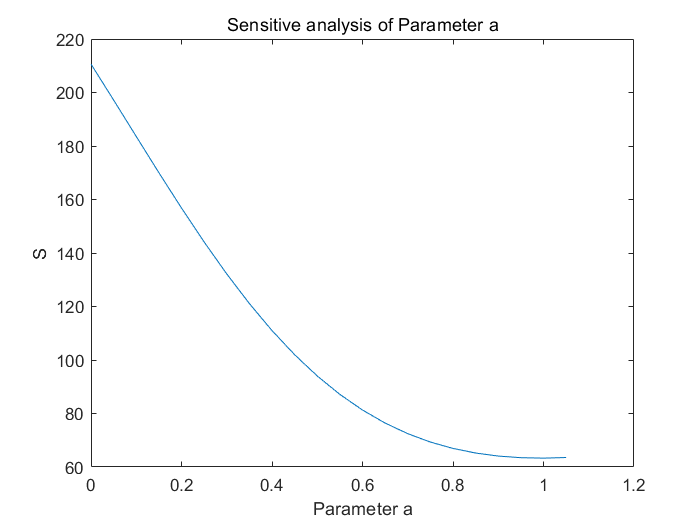
\includegraphics[width=0.7\linewidth]{./figures/Sen_a.png}
	\caption{The sensitive of parament: a}
	\label{F 8.1}
\end{minipage}\hfill
	\begin{minipage}[t]{0.48\linewidth}
\centering
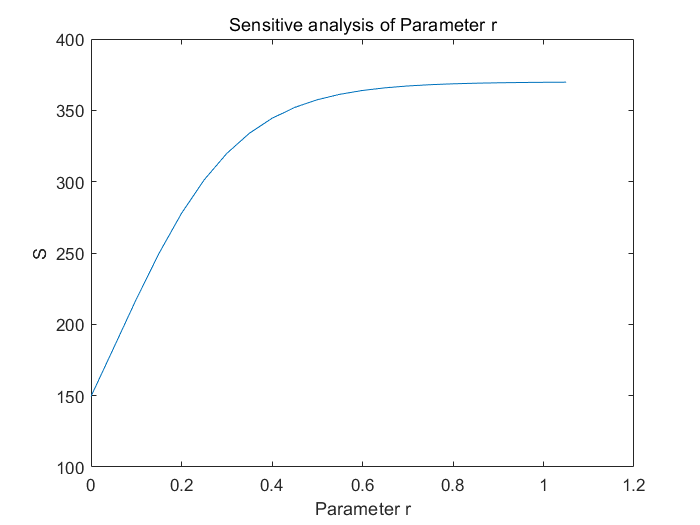
\includegraphics[width=0.7\linewidth]{./figures/sen_r.png}
\caption{The sensitive of parament: r
		}
\label{F 8.2}
\end{minipage}\hfill
\end{figure}
\begin{figure}[htbp]
	\centering
	\begin{minipage}[t]{0.48\linewidth}
	\centering
	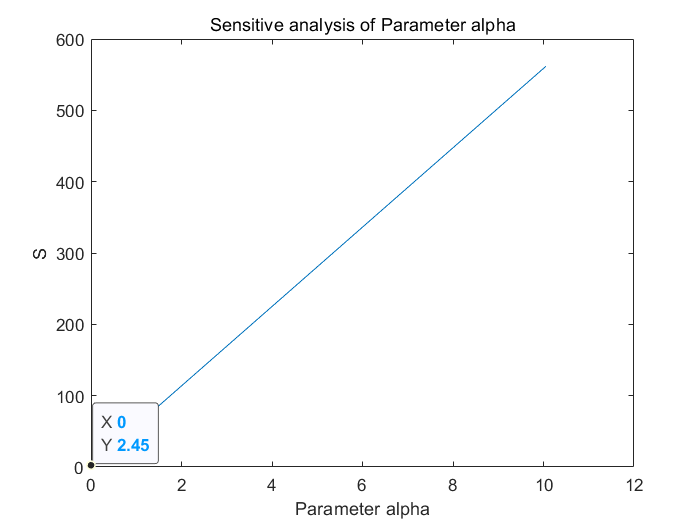
\includegraphics[width=0.7\linewidth]{./figures/sen_alpha.png}
	\caption{The sensitive of parament: $\alpha$}
	\label{F 1.1}
\end{minipage}\hfill
	\begin{minipage}[t]{0.48\linewidth}
\centering
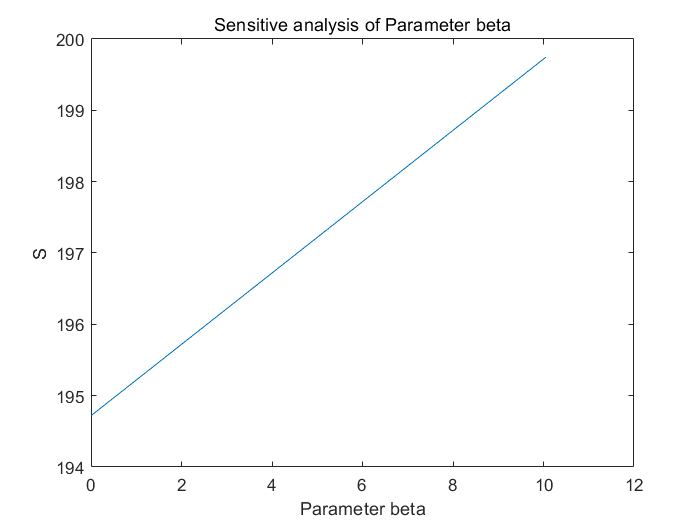
\includegraphics[width=0.7\linewidth]{./figures/sen_beta.png}
\caption{The sensitive of parament: $\beta$
		}
\label{F 1.2}
\end{minipage}\hfill
\end{figure}


\subsection{Conclussion}

Slight changes to the parameters a,r,$\alpha$ lead to a dramatic effect on output S. However, changing the parameter $\beta$ has essentially no effect on output S. We believe that it is because in the equation for output S, a is linear with respect to time t, and in our analysis S is obtained as a gain over a short period of time, so a change in the parameter $\beta$ in the image has little effect on output S. In general, however, although the sensitivity of $\beta$ is not high, the sensitivity of the other parameters a,r,$\alpha$ is high and in general the model has good sensitivity.

\section{Analysis of advantages and disadvantages}
\subsection{Advantages}
The model takes into account the differences between different areas in the region, using rasterisation to divide them into different regions and discussing them by region, reflecting the accuracy of the model.
The equilibrium model possesses broad applicability, yielding similar results when predicting species populations and economic benefits in different areas, reflecting consistency.
The evaluation model weighted the economic benefits and animal populations under different policies and the comparison yielded the best policy.
\subsection{Disadvantages}
The results of the evaluation model for different regions under the same policy are basically the same, which shows that the evaluation model is not accurate and objective enough. The introduction of hierarchical analysis could be considered for a more objective weighting analysis.

\section{Conclusion}

To investigate the effects of different policies on wildlife in different areas of the Maasai Mara, we first rasterised the Maasai Mara into three areas and then used an equilibrium model to investigate the effects of different policies on wildlife in one of these areas. The model was finally analysed for certainty, adaptability and sensitivity, and conclusions were drawn. Of all the areas in the Masai Mara, the policy of increasing the size of the reserve by limiting the livestock area provides the greatest benefit over the next 10 years, and applying the model to another reserve, the Serengeti, also proves to be the best policy. In addition, we conducted a data comparison and concluded that it matched the historical data. Finally, based on the findings of our model, we wrote a non-technical report to the Kenyan Tourism and Wildlife Committee.

\newpage()
\newpage()
\newpage()



\begin{thebibliography}{99}
\bibitem{1}  Bhola, N., Ogutu, J. O., Said, M. Y., Piepho, H. P., \& Olff, H. (2012). The distribution of large herbivore hotspots in relation to environmental and anthropogenic correlates in the Mara region of Kenya. Journal of Animal Ecology, 81(6), 1268-1287.
\bibitem{2}  Wei, Qingfeng. (2022). Research on ecological sensitivity analysis and conservation zoning of Guangxi Dayao Mountain Scenic Area (Master's thesis, Guangxi University). https://kns.cnki.net/KCMS/detail/detail.aspx?dbname=CMFDTEMP\&filename=1022727320.nh
\bibitem{3} Ogutu, J. O., Owen‐Smith, N., Piepho, H. P., \& Said, M. Y. (2011). Continuing wildlife population declines and range contraction in the Mara region of Kenya during 1977–2009. Journal of Zoology, 285(2), 99-109.
\bibitem{4} \url{https://data.worldbank.org/indicator/AG.LND.TOTL.K2?locations=KE}
\bibitem{5} \url{https://tradingeconomics.com/kenya/gdp}
\bibitem{6} \url{https://www.statista.com/statistics/1190810/tourism-receipts-in-tanzania/}
\bibitem{7} \url{https://data.worldbank.org/indicator/AG.LND.TOTL.K2?locations=KE}
\bibitem{8} \url{https://tradingeconomics.com/tanzania/gdp-from-agriculture}
\bibitem{9} \url{https://data. K2?locations=KE}
\bibitem{10} \url{Sinclair, A. R. E., Fryxell, J. M., Hilborn, R., \& Thirgood, S. (2007). Long-Term Ecosystem Dynamics in the Serengeti: Lessons for Conservation. (Conservation Biology, 21(3), 580-590.).}
\end{thebibliography}

\begin{appendices}
	
\section{Code}

\subsection{Logistic}

t0=0;
tfinal=35; % define the duration of year
xm=84;%number of environmental load-bearing specie
x0=0.5*84;%initial number of animals


[t, xt0]= ode45(@sunfun0, [t0 tfinal ], x0); %caculate in differential equation by ode45
[t, xt3]= ode45(@sunfun3, [t0 tfinal ], x0);
[t, xt5]= ode45(@sunfun5, [t0 tfinal ], x0);

plot(t,xt0)
hold on;
plot(t,xt3)
plot(t,xt5)
 xlabel('Year');
 ylabel('Numbers');
 legend('Zone A','Zone B','Zone C');

function xdot1=sunfun0(t,x)
xdot1=0.07*x*(1-x/(1.25*84));
end

function xdot1=sunfun3(t,x)
xdot1=0.07*x*(1-x/(1.875*84));
end

function xdot1=sunfun5(t,x)
xdot1=0.07*x*(1-x/(2.5*84));
end

\subsection{Economic}

syms x t    
alpha=3.5; %Annual tourism income earned per square kilometre of land
beta=4.9; %Annual agricultural income that can be earned per square kilometre of land
r=0.07;%Natural growth rate of species
x0=42;%Number of species per square kilometre, with maximum animal growth at the beginning of the rainy season
xm=210;% number of environmental load-bearing species, xm varies from zone to zone
a=-0.1;% annual human encroachment on protected areas for agricultural production assumed here to be -0.1%


syms X(t)    %solving differential equation of Benefits and Numbers
eqn = diff(X,t) ==r*X*(1-X/xm)*(1-a*t);  
con = X(0) == 42;
Xs= dsolve(eqn,con);


s=alpha*(Xs)+a*t*beta;
subplot(211)    %plot the Benift-Year diagram
 fplot(s,[0 1000]);
 xlabel('Year');
 ylabel('Benifit');

s1=Xs;         %plot the Species Numbers-Year diagram
subplot(212)
fplot(s1,[0 1000]);
 xlabel('Year');
 ylabel('Numbers');

s2=xm/(1+(xm/x0-1)*exp(-r*t));
%subplot(313)
%fplot(s2,[0 50]);
 %xlabel('Year');
 %ylabel('animal numbers(human unresrticted)');

%Changing r values Affects species growth rate (giant)
% change in xm value affects species population max
%a value increases, the number of years required to reach the species population maximum is advanced, the species population maximum decreases

\subsection{Entropy weighting method}

M1=[212
198
184
240
105
122

]
M2=[60
55
51
70
34
34


]

M=[M1,M2];

[raw,col]=size(M);% returns the number of elements in the row of the matrix

%Normalisation of matrices
 sums=sum(M,1);
 for i=1:raw
     for j=1:col
         M(i,j)=M(i,j)/sums(j);
   
     end
 end
% output is M which is the normalised decision matrix

%Calculation of weighting percentages
k=1/log(raw);
E=zeros(1,col);
for i=1:raw
    for j=1:col
     E(j)=E(j)-k*M(i,j)*log(M(i,j));
    end
end
% output E as entropy
F=ones(1,col)-E;
% Calculation of influence weights between individual elements
w=zeros(1,col);
for j=1:col
    w(j)=F(j)/sum(F);
end
% Introduce a v-weighted sum, the larger the weighted sum the more this option is recommended
v=M*w';
[raww,coll]=size(v);% returns the number of elements in the row of the matrix
% Returns the entropy weights of each element of the w matrix 
% and returns the v matrix to obtain the most recommended solution
w
v
% Draw a scatter plot of the options and weighted sums to visualise the most recommended options
method=[1:1:raww];
scatter(method,v);
xlabel('methodN')
ylabel('weighted sum')



\end{appendices}






\end{document}
%%
%% This work consists of these files mcmthesis.dtx,
%%                                   figures/ and
%%                                   code/,
%% and the derived files             mcmthesis.cls,
%%                                   mcmthesis-demo.tex,
%%                                   README,
%%                                   LICENSE,
%%                                   mcmthesis.pdf and
%%                                   mcmthesis-demo.pdf.
%%
%% End of file `mcmthesis-demo.tex'.
